\documentclass[tikz,border=2pt]{standalone}
\usepackage{tikz}
\usetikzlibrary{arrows.meta, positioning, calc, fit, backgrounds}

\definecolor{shared}{HTML}{E8EFF5}
\definecolor{cmbmod}{HTML}{F8D7DA}
\definecolor{galmod}{HTML}{E2D4F0}
\definecolor{outputbg}{HTML}{F5F5F5}
\definecolor{prmod}{HTML}{DCEDC8}       % primordial — light green, distinct

\begin{document}
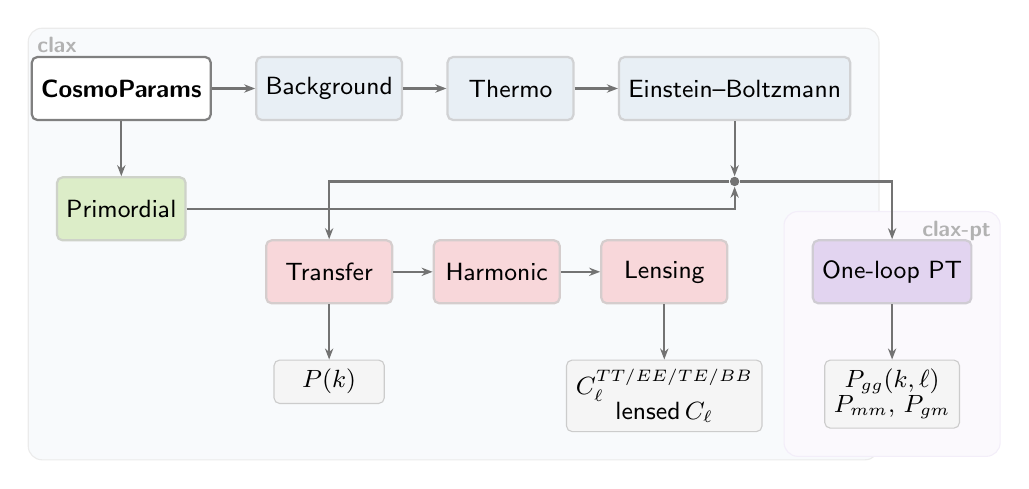
\begin{tikzpicture}[
    every node/.style={font=\sffamily},
    mod/.style={
        rectangle, rounded corners=2pt, draw=#1!60!black!40, fill=#1,
        thick, minimum width=1.6cm, minimum height=0.8cm, align=center,
        font=\sffamily\small
    },
    mod/.default=shared,
    outputbox/.style={
        rectangle, rounded corners=2pt, draw=black!20, fill=outputbg,
        minimum width=1.4cm, minimum height=0.55cm, align=center,
        font=\sffamily\small
    },
    flow/.style={-{Stealth[length=4pt, width=3pt]}, thick, black!55},
    dot/.style={circle, fill=black!55, inner sep=1.2pt},
]

% ===== Row 1: Boltzmann chain =====
\node[mod, draw=black!50, fill=white, font=\sffamily\small\bfseries]
    (params) {CosmoParams};

\node[mod, right=0.55cm of params] (bg) {Background};
\node[mod, right=0.55cm of bg] (th) {Thermo};
\node[mod, right=0.55cm of th, minimum width=2.0cm] (eb) {Einstein--Boltzmann};

% Primordial: independent of EB, depends only on CosmoParams
% Place it below the main row, between params and the fork
\node[mod=prmod, below=0.7cm of params] (pr) {Primordial};

% Row 1 arrows
\draw[flow] (params) -- (bg);
\draw[flow] (bg) -- (th);
\draw[flow] (th) -- (eb);

% CosmoParams also feeds Primordial directly
\draw[flow] (params) -- (pr);

% ===== Fork point: EB output splits into two branches =====
\node[dot, below=0.7cm of eb] (fork) {};
\draw[flow] (eb) -- (fork);

% ===== Row 2 left: CMB branch =====
\node[mod=cmbmod, below=1.5cm of bg] (tr) {Transfer};
\node[mod=cmbmod, right=0.5cm of tr] (hr) {Harmonic};
\node[mod=cmbmod, right=0.5cm of hr] (le) {Lensing};

% ===== Row 2 right: Galaxy branch =====
\node[mod=galmod, below=1.5cm of eb, xshift=2.0cm] (ept) {One-loop PT};

% Fork → both branches
\draw[flow] (fork) -| (tr);
\draw[flow] (fork) -| (ept);

% Primordial merges into the fork line — feeds both branches
% Draw Primordial → fork (joins the vertical from EB)
\draw[flow] (pr) -| (fork);

% ===== Row 3: Outputs =====
\node[outputbox, below=0.7cm of tr] (pkout) {$P(k)$};
\node[outputbox, below=0.7cm of le] (clout) {$C_\ell^{TT/EE/TE/BB}$\\[-2pt]{\small lensed\,$C_\ell$}};
\node[outputbox, below=0.7cm of ept] (pgout) {$P_{gg}(k,\ell)$\\[-2pt]{\small $P_{mm},\,P_{gm}$}};

% CMB chain
\draw[flow] (tr) -- (hr);
\draw[flow] (hr) -- (le);

% Outputs
\draw[flow] (tr) -- (pkout);
\draw[flow] (le) -- (clout);
\draw[flow] (ept) -- (pgout);

% ===== Background shading =====
\begin{scope}[on background layer]
    % clax region
    \node[fit=(bg)(th)(eb)(pr)(tr)(hr)(le)(pkout)(clout),
          draw=black!8, fill=shared!30, rounded corners=5pt,
          inner sep=10pt,
          label={[font=\sffamily\footnotesize\bfseries, text=black!30,
                  anchor=north west]north west:\textsc{clax}}] {};
    % clax-pt region
    \node[fit=(ept)(pgout),
          draw=galmod!40, fill=galmod!15, rounded corners=5pt,
          inner sep=10pt,
          label={[font=\sffamily\footnotesize\bfseries, text=black!30,
                  anchor=north east]north east:\textsc{clax-pt}}] {};
\end{scope}

\end{tikzpicture}
\end{document}
